% Standalone figure: run make in this directory to build PDF and SVG.
\documentclass[11pt,tikz,border=0pt]{standalone}
\usepackage{fontspec}
\IfFontExistsTF{Helvetica Neue Light}{
  \setsansfont{Helvetica Neue Light}[BoldFont={Helvetica Neue Medium}]
  \newfontfamily\vnmedium{Helvetica Neue Medium}
}{
  \setsansfont{TeX Gyre Heros}
  \newcommand{\vnmedium}{\bfseries}
}
\renewcommand{\familydefault}{\sfdefault}
\usepackage{amsmath,amssymb,mathtools}
\usepackage{unicode-math}
\setmathfont{latinmodern-math.otf}
\usetikzlibrary{arrows.meta,calc,positioning}
\definecolor{vnslideink}{HTML}{333333}
\definecolor{vnslidebody}{HTML}{5E5E5E}
\definecolor{vnaccent}{HTML}{FF644E}
\definecolor{vnslidelink}{HTML}{579ACA}
\pagecolor{white}
\tikzset{
  graphvertex/.style={draw=vnslideink,circle,fill=white,line width=0.7pt,
    minimum size=7mm,inner sep=0pt,font=\small\vnmedium},
  graphedge/.style={draw=vnslidebody,line width=0.8pt},
  grapharrow/.style={draw=vnslidebody,line width=0.8pt,-{Latex[length=2.5mm]}},
  graphaccent/.style={draw=vnaccent,line width=1.2pt,-{Latex[length=2.5mm]}},
}

\begin{document}
\color{vnslidebody}
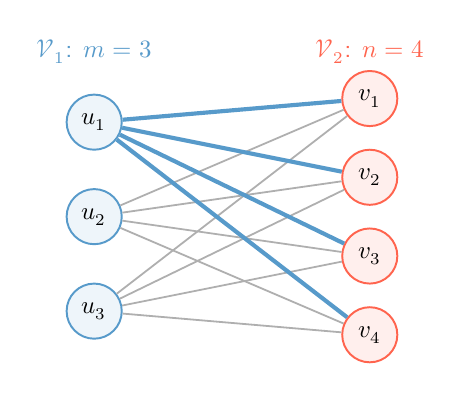
\begin{tikzpicture}[x=1cm,y=1cm]
        \node[font=\small\vnmedium,text=vnslidelink] at (0,2.1) {$\mathcal V_1$: $m=3$};
        \node[font=\small\vnmedium,text=vnaccent] at (3.5,2.1) {$\mathcal V_2$: $n=4$};
        \foreach \i/\y in {1/1.2,2/0,3/-1.2}
          {\node[graphvertex,draw=vnslidelink,fill=vnslidelink!10] (u\i) at (0,\y) {$u_{\i}$};}
        \foreach \j/\y in {1/1.5,2/0.5,3/-0.5,4/-1.5}
          {\node[graphvertex,draw=vnaccent,fill=vnaccent!10] (v\j) at (3.5,\y) {$v_{\j}$};}
        \foreach \i in {2,3}
          {\foreach \j in {1,...,4} {\draw[draw=vnslidebody!50,line width=0.65pt] (u\i)--(v\j);}}
        \foreach \j in {1,...,4}
          {\draw[draw=vnslidelink,line width=1.5pt] (u1)--(v\j);}
        \path[use as bounding box] (-0.7,-1.9) rectangle (4.2,2.4);
      \end{tikzpicture}
\end{document}
